Finally, we try to go one step further with the network, making it simpler without losing much performance.
Given that we have a trained model with over 75\%, we can use \emph{knowledge distillation}
\footnote{"Knowledge Distillation and Student-Teacher Learning for Visual Intelligence: A Review and
New Outlooks", available at \href{https://arxiv.org/pdf/2004.05937.pdf}{https://arxiv.org/pdf/2004.05937.pdf}}
on it, defining its role as a \emph{teacher} and creating a much simpler \emph{student} model.\\
Teacher network:
\begin{center}
    \begin{verbatim}
        Model: "teacher"
        _________________________________________________________________
        Layer (type)                 Output Shape              Param #   
        =================================================================
        conv2d (Conv2D)              (None, 32, 32, 32)        320       
        _________________________________________________________________
        batch_normalization (BatchNo (None, 32, 32, 32)        128       
        _________________________________________________________________
        conv2d_1 (Conv2D)            (None, 32, 32, 32)        9248      
        _________________________________________________________________
        batch_normalization_1 (Batch (None, 32, 32, 32)        128       
        _________________________________________________________________
        max_pooling2d (MaxPooling2D) (None, 16, 16, 32)        0         
        _________________________________________________________________
        dropout (Dropout)            (None, 16, 16, 32)        0         
        _________________________________________________________________
        conv2d_2 (Conv2D)            (None, 16, 16, 64)        18496     
        _________________________________________________________________
        batch_normalization_2 (Batch (None, 16, 16, 64)        256       
        _________________________________________________________________
        conv2d_3 (Conv2D)            (None, 16, 16, 64)        36928     
        _________________________________________________________________
        batch_normalization_3 (Batch (None, 16, 16, 64)        256       
        _________________________________________________________________
        max_pooling2d_1 (MaxPooling2 (None, 8, 8, 64)          0         
        _________________________________________________________________
        dropout_1 (Dropout)          (None, 8, 8, 64)          0         
        _________________________________________________________________
        conv2d_4 (Conv2D)            (None, 8, 8, 128)         73856     
        _________________________________________________________________
        batch_normalization_4 (Batch (None, 8, 8, 128)         512       
        _________________________________________________________________
        conv2d_5 (Conv2D)            (None, 8, 8, 128)         147584    
        _________________________________________________________________
        batch_normalization_5 (Batch (None, 8, 8, 128)         512       
        _________________________________________________________________
        max_pooling2d_2 (MaxPooling2 (None, 4, 4, 128)         0         
        _________________________________________________________________
        dropout_2 (Dropout)          (None, 4, 4, 128)         0         
        _________________________________________________________________
        flatten (Flatten)            (None, 2048)              0         
        _________________________________________________________________
        dense (Dense)                (None, 128)               262272    
        _________________________________________________________________
        dense_1 (Dense)              (None, 10)                1290      
        =================================================================
        Total params: 551,786
        Trainable params: 550,890
        Non-trainable params: 896
        _________________________________________________________________
    \end{verbatim}
\end{center}
Student network:
\begin{center}
    \begin{verbatim}
        Model: "student"
        _________________________________________________________________
        Layer (type)                 Output Shape              Param #   
        =================================================================
        conv2d_6 (Conv2D)            (None, 32, 32, 32)        320       
        _________________________________________________________________
        batch_normalization_6 (Batch (None, 32, 32, 32)        128       
        _________________________________________________________________
        conv2d_7 (Conv2D)            (None, 32, 32, 32)        9248      
        _________________________________________________________________
        batch_normalization_7 (Batch (None, 32, 32, 32)        128       
        _________________________________________________________________
        max_pooling2d_3 (MaxPooling2 (None, 16, 16, 32)        0         
        _________________________________________________________________
        dropout_3 (Dropout)          (None, 16, 16, 32)        0         
        _________________________________________________________________
        flatten_1 (Flatten)          (None, 8192)              0         
        _________________________________________________________________
        dense_2 (Dense)              (None, 10)                81930     
        =================================================================
        Total params: 91,754
        Trainable params: 91,626
        Non-trainable params: 128
        _________________________________________________________________
    \end{verbatim}
\end{center}
For the implementation, we use as a guide the Keras documentation.\footnote{\href{https://keras.io/examples/vision/knowledge\_distillation/}{https://keras.io/examples/vision/knowledge\_distillation/}}
The experiment consists in training the student model both from the input and from the weights learned by the teacher model.
In order to achieve this, the loss function to minimize by the student, other than the Cross Entropy for the teacher, is KL Divergence
\footnote{\href{https://www.tensorflow.org/api\_docs/python/tf/keras/losses/KLDivergence}{https://www.tensorflow.org/api\_docs/python/tf/keras/losses/KLDivergence}},
which considers both results and leads the student to learn from them.\\
Unfortunately, our experimenting results are not very successful, given that training our student model for itself gives us almost the same results than the distilled version.
We tried different values for the distiller's parameters (temperature, alpha), as well as different layers dispositions for the student, always with similar results
(even getting worse accuracies, but both alike). Given a teacher with approximately 75\% accuracy, we obtain a student with approximately 58\% accuracy:
\begin{center}
    \captionsetup{type=figure}
    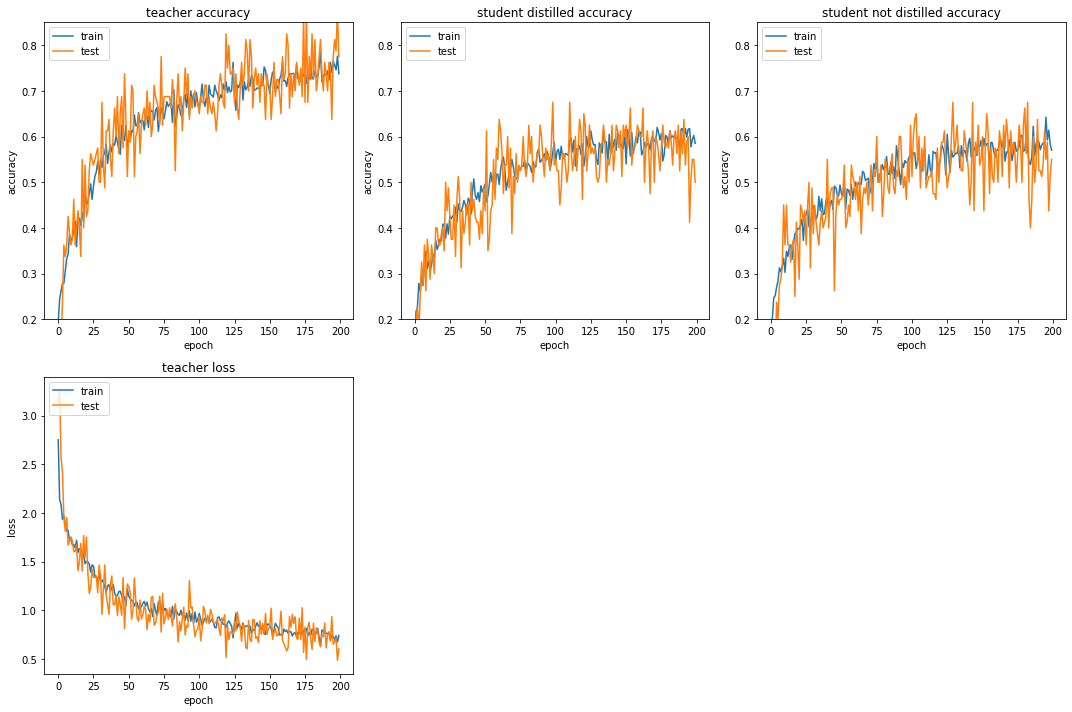
\includegraphics[width=400px]{sections/exp-1/images/distiller-acc.png}
    \captionof{figure}{Distilling - Loss \& Accuracy}
\end{center}